\documentclass[12pt,a4paper]{report}
% Condensed Software Construction (CS23432) report -- same house format as the internship report.
\usepackage[a4paper,top=2.3cm,bottom=2.2cm,left=2.8cm,right=2.3cm]{geometry}
\usepackage[T1]{fontenc}
\usepackage{newtxtext,newtxmath}
\usepackage{graphicx}
\newcommand{\Usefont}[1]{\fontfamily{#1}\selectfont}
\usepackage{setspace}
\usepackage{array}
\usepackage{booktabs}
\usepackage{tabularx}
\usepackage{subcaption}
\usepackage{enumitem}
\usepackage{titlesec}
\usepackage{fancyhdr}
\usepackage{xcolor}
\usepackage{colortbl}
\usepackage{tikz}
\usetikzlibrary{shapes.geometric,shapes.multipart,arrows.meta,positioning,fit,calc}
\usepackage{float}
\usepackage{caption}
\usepackage{microtype}
\usepackage{listings}
\usepackage{mdframed}
\usepackage{needspace}
\usepackage[hidelinks]{hyperref}

\setlength{\headheight}{16pt}

\definecolor{navy}{RGB}{0,0,0}
\definecolor{navysoft}{RGB}{60,60,60}
\definecolor{steel}{RGB}{95,95,95}
\definecolor{rulegray}{RGB}{150,150,150}
\definecolor{rowgray}{RGB}{240,240,240}
\definecolor{codebg}{RGB}{247,247,247}

\setstretch{1.12}
\setlength{\parindent}{1.5em}
\setlist{itemsep=1pt,parsep=0pt,topsep=3pt}
\captionsetup{font=small,labelfont={bf,color=navy},labelsep=period}
\captionsetup[figure]{name=Fig.}
\captionsetup[table]{name=Table}

% Chapter style from the internship report, compacted so chapters flow without page breaks.
\titleformat{\section}{\normalfont\large\bfseries\color{navy}}{\thesection}{0.6em}{}
\titleformat{\subsection}{\normalfont\normalsize\bfseries\color{navysoft}}{\thesubsection}{0.6em}{}
\titlespacing*{\section}{0pt}{9pt}{3pt}
\titlespacing*{\subsection}{0pt}{6pt}{2pt}
\makeatletter
\renewcommand{\@makechapterhead}[1]{{\parindent\z@\raggedright\normalfont
  \Large\bfseries\color{navy}\MakeUppercase{Chapter~\thechapter\quad #1}\par
  \vspace{2pt}{\color{navysoft}\rule{\linewidth}{1.2pt}}\par\vspace{8pt}}}
\renewcommand\chapter[1]{\par\needspace{8\baselineskip}\addvspace{10pt}\refstepcounter{chapter}\setcounter{section}{0}\@makechapterhead{#1}}
\makeatother

\pagestyle{fancy}
\fancyhf{}
\renewcommand{\headrulewidth}{0pt}
\fancyhead[L]{\small\color{steel}\itshape 2116241901035}
\fancyhead[R]{\small\color{steel}\itshape CS23432 Software Construction}
\fancyhead[C]{\color{navy}\rule[-6pt]{\textwidth}{0.4pt}}
\fancyfoot[C]{\small\color{navy}\textbf{\thepage}}
\fancypagestyle{plain}{\fancyhf{}\fancyfoot[C]{\small\color{navy}\textbf{\thepage}}\renewcommand{\headrulewidth}{0pt}}

\newcolumntype{L}[1]{>{\raggedright\arraybackslash}p{#1}}
\newcolumntype{C}[1]{>{\centering\arraybackslash}p{#1}}
\newcommand{\hd}[1]{{\color{white}\bfseries #1}}
\renewcommand{\arraystretch}{1.2}
\newcommand{\headrow}{\rowcolor{navy}}
\newcommand{\code}[1]{\texttt{\small #1}}

\lstset{basicstyle=\ttfamily\scriptsize,backgroundcolor=\color{codebg},frame=single,
  rulecolor=\color{rulegray},breaklines=true,columns=fullflexible,showstringspaces=false,
  xleftmargin=2pt,xrightmargin=2pt}

\newmdenv[backgroundcolor=rowgray,linecolor=navy,linewidth=1pt,
  innerleftmargin=10pt,innerrightmargin=8pt,innertopmargin=6pt,innerbottommargin=6pt,
  skipabove=6pt,skipbelow=6pt]{keybox}

% UML helper: class box with name / attributes / operations
\tikzset{
  cls/.style={rectangle split,rectangle split parts=3,draw=black,fill=white,font=\scriptsize,
    text width=3.35cm,inner sep=2.5pt,align=left,rectangle split part fill={rowgray,white,white}},
  gen/.style={-{Triangle[open,length=5pt,width=5pt]},thick},
  assoc/.style={-{Stealth[length=4pt]},thick},
  lay/.style={rectangle,draw=black,rounded corners=2pt,font=\scriptsize\bfseries,
    minimum height=0.8cm,text width=3.3cm,align=center,fill=rowgray},
}

\begin{document}

% ==================== TITLE PAGE ======================
\thispagestyle{empty}
\begin{titlepage}
\begin{center}
{\Usefont{ppl}\Large\bfseries RAJALAKSHMI ENGINEERING COLLEGE}\\[2pt]
\normalsize THANDALAM, CHENNAI -- 602105\\[24pt]
{\Usefont{ppl}\Large\bfseries CS23432 / SOFTWARE CONSTRUCTION}\\[2pt]
(LAB ORIENTED THEORY COURSE)\\[10pt]
\normalsize Project Report on\\[6pt]
{\Usefont{ppl}\large\bfseries Design, Testing and CI/CD Analysis of the\\
Spring PetClinic Reference Application}\\[24pt]
\normalsize Submitted by\\[6pt]
{\Usefont{ppl}\large\bfseries N. HARISH VIDYARTH}\\
Register No.: 2116241901035\\[4pt]
III Year -- B.E. CSE (Cyber Security)\\[22pt]
\normalsize \textit{in partial fulfillment of the award of the degree of}\\[12pt]
{\Usefont{ppl}\large\bfseries BACHELOR OF ENGINEERING}\\
\normalsize \textit{in}\\
{\Usefont{ppl}\large\bfseries COMPUTER SCIENCE AND ENGINEERING}\\
{\Usefont{ppl}\large\bfseries (CYBER SECURITY)}\\[18pt]
\normalsize\bfseries ACADEMIC YEAR: 2026 -- 2027\\[8pt]
\bfseries October 2026\\[\stretch{1}]

\includegraphics[scale=1.3]{assets/logo.jpg}\\[\stretch{1}]
\footnotesize\bfseries DEPARTMENT OF COMPUTER SCIENCE AND ENGINEERING (CYBER SECURITY)\\
\bfseries RAJALAKSHMI ENGINEERING COLLEGE, CHENNAI
\end{center}
\end{titlepage}

% ==================== CERTIFICATE ======================
\thispagestyle{empty}
\begin{center}
{\Usefont{ppl}\Large\bfseries BONAFIDE CERTIFICATE}
\end{center}
\vspace{1.2cm}
\noindent Certified that this project report \textbf{``DESIGN, TESTING AND CI/CD ANALYSIS OF THE
SPRING PETCLINIC REFERENCE APPLICATION''} is the bonafide work of \textbf{``N.\ HARISH VIDYARTH''}
(Register No.\ 2116241901035), who carried out the project work for the course
\textbf{CS23432 -- Software Construction} under my supervision.
\vspace{3.2cm}

\begin{flushright}
\begin{minipage}{0.5\textwidth}
\textbf{SIGNATURE}\\[1.2cm]
\textbf{Ms.\ Rupmala R}\\
Course Faculty, CS23432\\
Dept.\ of Computer Science and Engineering (Cyber Security)\\
Rajalakshmi Engineering College, Chennai
\end{minipage}
\end{flushright}
\vspace{2.6cm}
\noindent\textbf{Submitted for the Practical Examination held on} \underline{\hspace{4.5cm}}
\vspace{2.2cm}
\begin{flushright}\textbf{EXAMINER}\hspace{1.2cm}\end{flushright}
\clearpage

% ==================== MAIN MATTER ======================
\pagenumbering{arabic}
\setcounter{page}{1}

\chapter{Introduction and Software Selection}
\section{Aim}
To study, model and verify a well-engineered open-source application using the practices taught
in CS23432: requirements, system modelling, design principles, testing and continuous
integration.

\section{Why Spring PetClinic}
\textbf{Spring PetClinic} (\code{spring-projects/spring-petclinic}) is the Spring team's
canonical reference application for a veterinary clinic. It was chosen because it is
maintained by the framework authors, uses a clean layered MVC structure, has a real entity model,
ships a broad automated test suite and a GitHub Actions workflow, and builds with a single
command. All facts below were read from the cloned source at commit
\code{500158f}.

\begin{table}[H]\centering\small
\begin{tabular}{L{3.6cm} L{9.6cm}}
\headrow\hd{Item} & \hd{Detail (from the repository)} \\
Stack & Spring Boot 4.1.0, Java 17, Spring MVC, Spring Data JPA, Thymeleaf \\
\rowcolor{rowgray}
Packages & \code{model}, \code{owner}, \code{vet}, \code{system} under
\code{org.springframework.samples.petclinic} \\
Build & Maven (\code{pom.xml}) and Gradle; Maven wrapper included \\
\rowcolor{rowgray}
CI & GitHub Actions: \code{maven-build.yml}, \code{gradle-build.yml},
\code{deploy-and-test-cluster.yml} \\
Tests & 19 test classes: 18 upstream plus \code{PetTests} added in this work \\
\end{tabular}
\caption{Project profile.}
\end{table}

\chapter{Requirements}
Requirements follow the Agile hierarchy of the course (theme $\rightarrow$ epic $\rightarrow$
story). The theme is \emph{Run a veterinary clinic}; the stories below were derived from the
controllers and views actually present in the application.

\begin{table}[H]\centering\small
\begin{tabular}{C{0.9cm} L{2.2cm} L{6.6cm} C{1.7cm}}
\headrow\hd{ID} & \hd{Epic} & \hd{User story} & \hd{Type} \\
US1 & Owners & As a receptionist I can search owners by last name so I find a client quickly. & FR \\
\rowcolor{rowgray}
US2 & Owners & As a receptionist I can register and edit an owner with address, city and telephone. & FR \\
US3 & Pets & As a receptionist I can add a pet with name, birth date and type to an owner. & FR \\
\rowcolor{rowgray}
US4 & Visits & As a vet I can record a visit (date, description) against a pet. & FR \\
US5 & Vets & As a client I can view veterinarians and their specialties. & FR \\
US6 & Pets & As a vet I can see each pet's age in years on the owner page (added in this work). & FR \\
\rowcolor{rowgray}
NF1 & Quality & Invalid input (blank name, bad telephone, future birth date) is rejected with a message. & NFR \\
NF2 & Delivery & Every change builds and passes all tests automatically in CI. & NFR \\
\rowcolor{rowgray}
NF3 & Portability & The app runs on an in-memory database with no setup, and on MySQL/PostgreSQL. & NFR \\
\end{tabular}
\caption{Functional (FR) and non-functional (NFR) user stories.}
\end{table}

\chapter{System Modelling and Design}
\section{Class Model}
The domain follows a small inheritance tree: \code{BaseEntity} (id) is extended by
\code{Person} (first and last name) and \code{NamedEntity} (name). \code{Owner} and \code{Vet}
specialise \code{Person}; \code{Pet}, \code{PetType} and \code{Specialty} specialise
\code{NamedEntity}. An owner holds many pets and a pet holds many visits.

\begin{figure}[H]\centering
\resizebox{0.97\linewidth}{!}{%
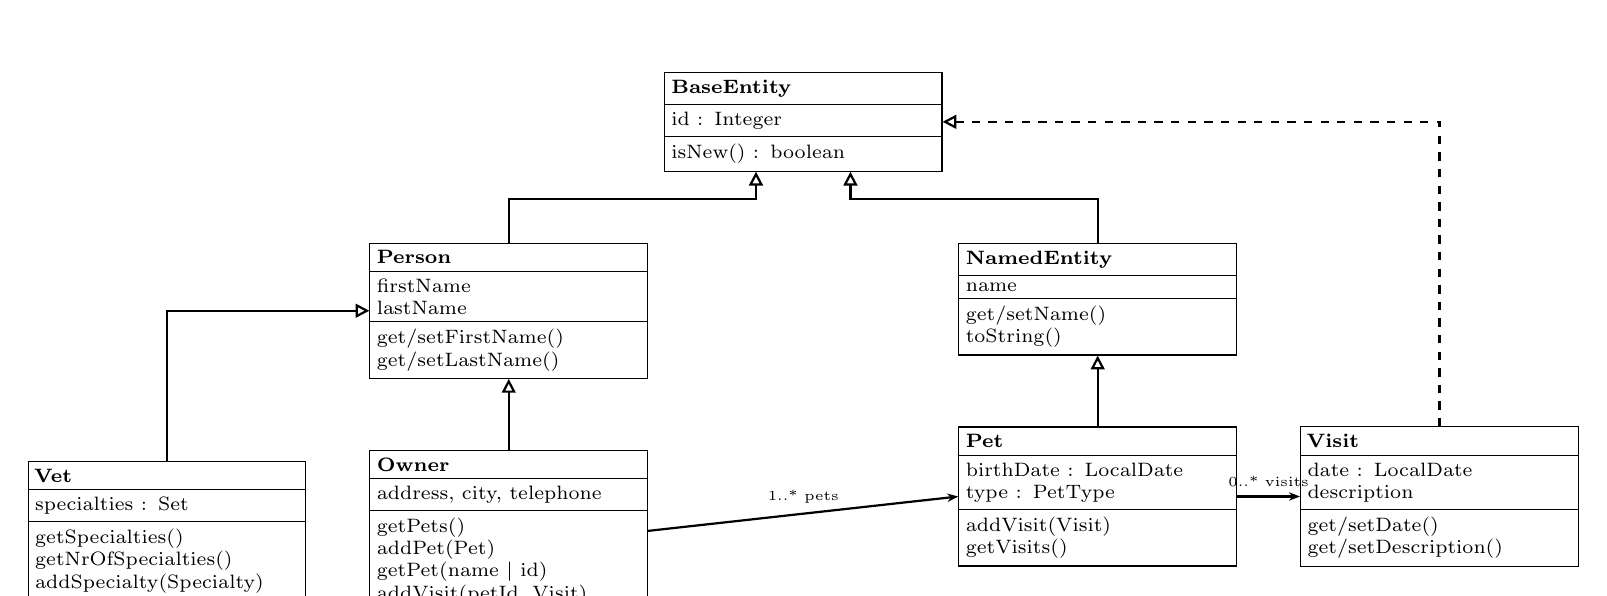
\begin{tikzpicture}[node distance=0.55cm and 0.7cm]
\node[cls] (base) {\textbf{BaseEntity}\nodepart{second}id : Integer\nodepart{third}isNew() : boolean};
\node[cls,below left=0.9cm and 0.2cm of base] (person) {\textbf{Person}\nodepart{second}firstName\\lastName\nodepart{third}get/setFirstName()\\get/setLastName()};
\node[cls,below right=0.9cm and 0.2cm of base] (named) {\textbf{NamedEntity}\nodepart{second}name\nodepart{third}get/setName()\\toString()};
\node[cls,below=0.9cm of person] (owner) {\textbf{Owner}\nodepart{second}address, city, telephone\nodepart{third}getPets()\\addPet(Pet)\\getPet(name \textbar\ id)\\addVisit(petId, Visit)};
\node[cls,left=0.8cm of owner] (vet) {\textbf{Vet}\nodepart{second}specialties : Set\nodepart{third}getSpecialties()\\getNrOfSpecialties()\\addSpecialty(Specialty)};
\node[cls,below=0.9cm of named] (pet) {\textbf{Pet}\nodepart{second}birthDate : LocalDate\\type : PetType\nodepart{third}addVisit(Visit)\\getVisits()};
\node[cls,right=0.8cm of pet] (visit) {\textbf{Visit}\nodepart{second}date : LocalDate\\description\nodepart{third}get/setDate()\\get/setDescription()};
\draw[gen] (person.north) |- ($(base.south)+(-0.6,-0.35)$) -- ($(base.south)+(-0.6,0)$);
\draw[gen] (named.north) |- ($(base.south)+(0.6,-0.35)$) -- ($(base.south)+(0.6,0)$);
\draw[gen] (owner.north) -- (person.south);
\draw[gen] (vet.north) |- ($(person.west)+(-0.45,0)$) -- (person.west);
\draw[gen] (pet.north) -- (named.south);
\draw[assoc] (owner.east) -- node[above,font=\tiny]{1..*\ pets} (pet.west);
\draw[assoc] (pet.east) -- node[above,font=\tiny]{0..*\ visits} (visit.west);
\draw[gen,dashed] (visit.north) |- ($(base.east)+(0.9,0)$) -- (base.east);
\end{tikzpicture}}
\caption{Domain class diagram derived from the \code{model}, \code{owner} and \code{vet} packages
(\code{PetType} and \code{Specialty} extend \code{NamedEntity}).}
\end{figure}

\section{Architecture (MVC)}
The application uses Spring MVC. Controllers handle HTTP requests, Spring Data repositories
(\code{OwnerRepository}, \code{VetRepository}, \code{PetTypeRepository}) isolate persistence,
Thymeleaf templates render views, and the JPA entities form the model.

\begin{figure}[H]\centering
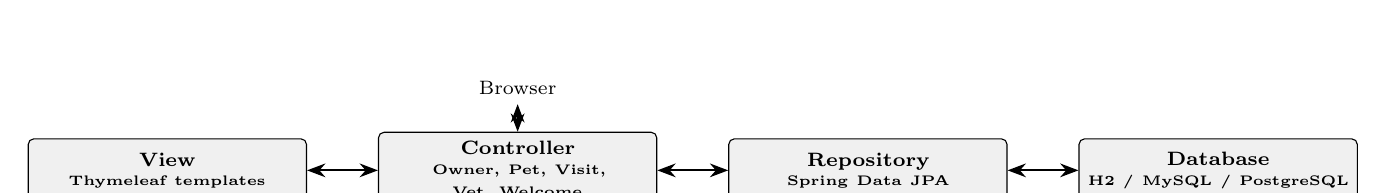
\begin{tikzpicture}[>=Stealth]
\node[lay] (v) {View\\[-1pt]\tiny Thymeleaf templates};
\node[lay,right=0.9cm of v] (c) {Controller\\[-1pt]\tiny Owner, Pet, Visit, Vet, Welcome};
\node[lay,right=0.9cm of c] (r) {Repository\\[-1pt]\tiny Spring Data JPA};
\node[lay,right=0.9cm of r] (d) {Database\\[-1pt]\tiny H2 / MySQL / PostgreSQL};
\node[above=0.35cm of c,font=\scriptsize] (b) {Browser};
\draw[<->,thick] (b) -- (c);
\draw[<->,thick] (v) -- (c);
\draw[<->,thick] (c) -- (r);
\draw[<->,thick] (r) -- (d);
\end{tikzpicture}
\caption{Layered MVC architecture of PetClinic.}
\end{figure}

\section{Interaction: Add a Visit (US4)}
\begin{figure}[H]\centering
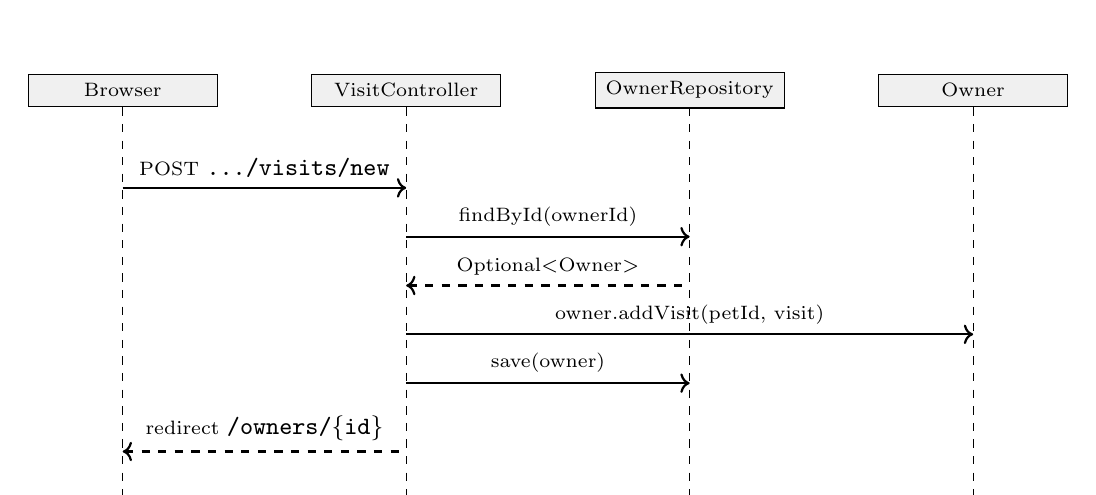
\begin{tikzpicture}[font=\scriptsize,x=3.6cm,y=-0.62cm]
\foreach \x/\n in {0/Browser,1/VisitController,2/OwnerRepository,3/Owner / Pet}{
  \node[draw,fill=rowgray,minimum width=2.4cm] (h\x) at (\x,0) {\n};
  \draw[dashed] (\x,0.35) -- (\x,8.6);}
\draw[->,thick] (0,2) -- node[above]{POST \code{.../visits/new}} (1,2);
\draw[->,thick] (1,3) -- node[above]{findById(ownerId)} (2,3);
\draw[<-,thick,dashed] (1,4) -- node[above]{Optional$<$Owner$>$} (2,4);
\draw[->,thick] (1,5) -- node[above]{owner.addVisit(petId, visit)} (3,5);
\draw[->,thick] (1,6) -- node[above]{save(owner)} (2,6);
\draw[<-,thick,dashed] (0,7.4) -- node[above]{redirect \code{/owners/\{id\}}} (1,7.4);
\end{tikzpicture}
\caption{Sequence diagram for recording a visit (validation errors re-render the form).}
\end{figure}

\chapter{SOLID Principles}
\begin{table}[H]\centering\small
\begin{tabular}{L{2.6cm} L{10.6cm}}
\headrow\hd{Principle} & \hd{Evidence in the code} \\
Single responsibility & Separate controllers per concern (\code{OwnerController},
\code{PetController}, \code{VisitController}, \code{VetController}); \code{PetValidator} only
validates; \code{PetTypeFormatter} only converts. \\
\rowcolor{rowgray}
Open/closed & Behaviour is extended through new Spring Data repository methods and formatters
without modifying entity classes. \\
Liskov substitution & \code{Owner} and \code{Vet} are usable wherever a \code{Person} is
expected; \code{Pet}, \code{PetType}, \code{Specialty} wherever a \code{NamedEntity} is. \\
\rowcolor{rowgray}
Interface segregation & Small repository interfaces (\code{OwnerRepository},
\code{VetRepository}, \code{PetTypeRepository}) expose only what each controller needs. \\
Dependency inversion & Controllers depend on repository \emph{interfaces}, injected by
Spring; implementations are generated at runtime. \\
\end{tabular}
\caption{SOLID principles mapped to PetClinic.}
\end{table}

\chapter{Testing and Verification}
\section{Test Strategy}
The suite mixes entity unit tests (\code{OwnerTests}, \code{VetTests}), validator tests,
MVC slice tests (\code{OwnerControllerTests}, \code{PetControllerTests},
\code{VisitControllerTests}, \code{VetControllerTests}), repository/service tests
(\code{ClinicServiceTests}), integration tests (\code{PetClinicIntegrationTests}) and a
concurrency test. Selected test cases mapped to the user stories:

\begin{table}[H]\centering\small
\begin{tabular}{C{0.9cm} L{4.6cm} L{6.6cm}}
\headrow\hd{Story} & \hd{Test class} & \hd{Expected behaviour verified} \\
US1 & \code{OwnerControllerTests} & Search by last name returns matching owners; unknown name shows none. \\
\rowcolor{rowgray}
US2 & \code{OwnerControllerTests} & Valid owner is saved and redirected; blank fields return the form with errors. \\
US3 & \code{PetControllerTests}, \code{PetValidatorTests} & Pet with valid name/type/date is created; invalid input rejected. \\
\rowcolor{rowgray}
US4 & \code{VisitControllerTests} & Visit is added and redirected; empty description rejected. \\
US5 & \code{VetControllerTests} & Vet list rendered with specialties. \\
\rowcolor{rowgray}
US6 & \code{PetTests} & Age is whole years; birthday counted; null for unknown or future birth date. \\
\end{tabular}
\caption{Traceability from user stories to automated tests.}
\end{table}

\section{Execution Result}
The suite was executed locally with \code{mvn test} (JDK 23 runtime, Maven build targeting
Java 17):

\begin{keybox}
\textbf{Result:} \texttt{Tests run: 85, Failures: 0, Errors: 0, Skipped: 2}\\\texttt{BUILD SUCCESS}\\
79 upstream tests plus 6 new \code{PetTests}. The two skipped tests are the container-based MySQL/PostgreSQL integration tests, which need Docker.
\end{keybox}

\section{Enhancement: Pet Age (US6)}
Beyond analysing the upstream code, one small feature was added to show the construction
workflow end to end (story $\rightarrow$ code $\rightarrow$ test $\rightarrow$ build). The owner
page now shows each pet's age in whole years.

\begin{itemize}[leftmargin=1.6em]
  \item \textbf{Model:} \code{Pet.getAgeInYears(LocalDate today)} returns whole years, or
        \code{null} when the birth date is unknown or in the future; a no-argument overload uses today's date.
        The \code{today} parameter keeps the logic testable without a clock.
  \item \textbf{View:} \code{ownerDetails.html} adds an Age row with the translated labels
        \code{age} and \code{years}, added to all ten \code{messages\_*.properties} files so
        \code{I18nPropertiesSyncTest} keeps passing.
  \item \textbf{Tests:} six \code{PetTests} cases (whole years, unfinished year, birthday, newborn,
        unknown date, future date). Full suite after the change: 85 run, 0 failures.
\end{itemize}

\begin{figure}[H]\centering
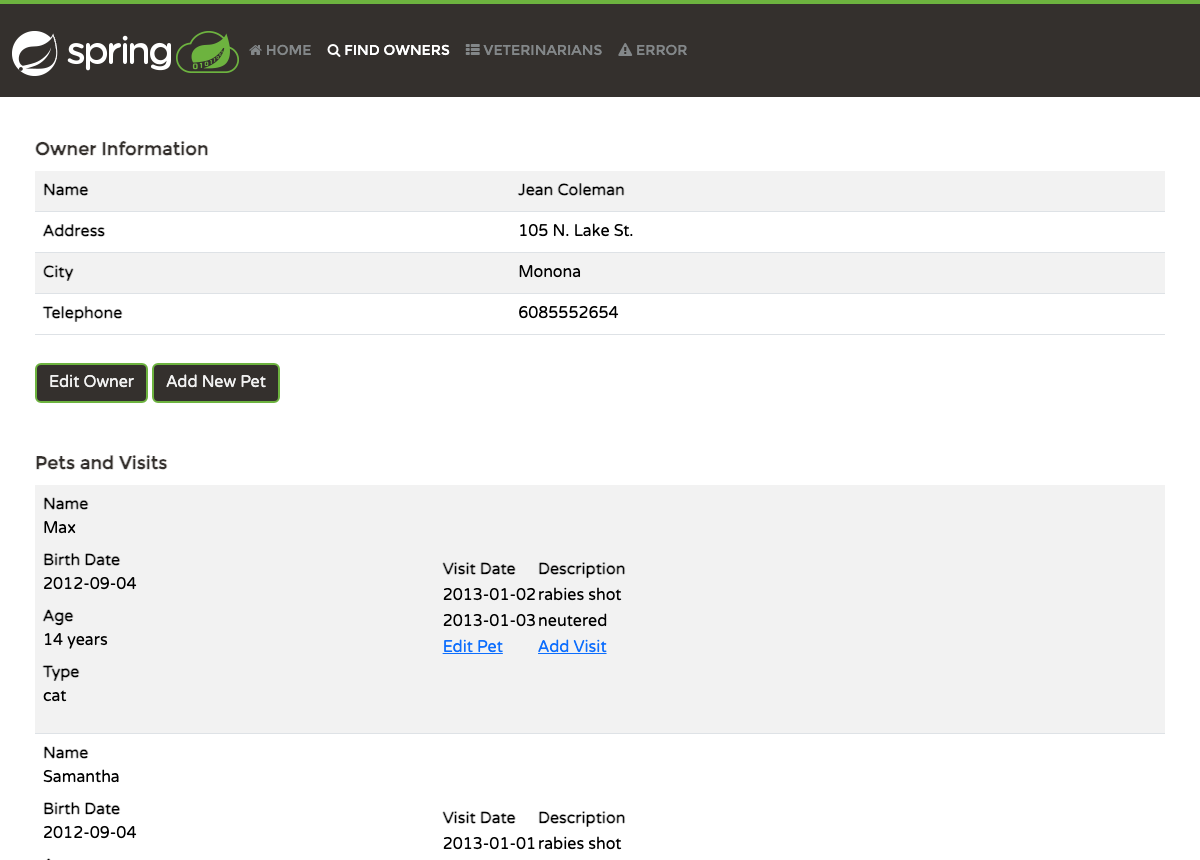
\includegraphics[width=0.6\linewidth]{assets/owner6_age.png}
\caption{Owner page after the enhancement: Max, born 2012-09-04, shows ``Age 14 years''.}
\end{figure}

\section{Running Application}
The application was also started (\code{mvn spring-boot:run}, in-memory H2 database) and its
pages were captured from a browser.

\begin{figure}[H]\centering
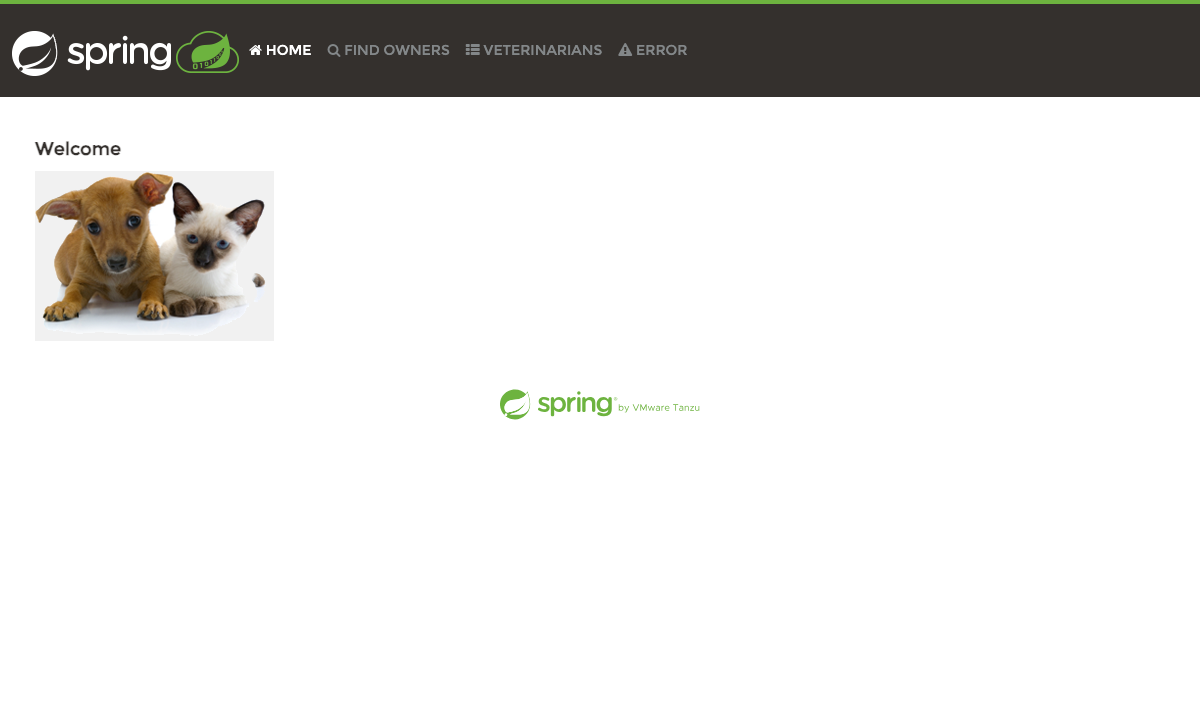
\includegraphics[width=0.5\linewidth]{assets/home.png}
\caption{PetClinic home page, running locally on an in-memory H2 database.}
\end{figure}

\chapter{Repository and Configuration Management}
\section{Repository Structure}
The source is managed in Git (Apache License 2.0). The layout below was read from the cloned
repository; templates, database scripts and tests sit beside the Java packages, which keeps
design, code and test artefacts in one tree.

\begin{lstlisting}
spring-petclinic/
  pom.xml, build.gradle, mvnw, gradlew       build definitions and wrappers
  .github/workflows/                         maven-build, gradle-build, deploy-and-test-cluster
  k8s/, docker-compose.yml                   deployment descriptors
  src/main/java/.../petclinic/
    model/   BaseEntity, NamedEntity, Person
    owner/   Owner, Pet, PetType, Visit + controllers, repositories, validator
    vet/     Vet, Specialty, Vets, VetController, VetRepository
    system/  WelcomeController, CrashController, CacheConfiguration, WebConfiguration
  src/main/resources/
    templates/ (owners, pets, vets, fragments)   Thymeleaf views
    db/ (h2, mysql, postgres)                    schema.sql + data.sql per database
    messages/                                    i18n bundles
  src/test/java/.../petclinic/               19 test classes mirroring the main packages
\end{lstlisting}

\section{Naming Conventions and Configuration}
Packages are organised by feature (\code{owner}, \code{vet}) rather than by technical layer;
controllers end in \code{Controller}, Spring Data interfaces in \code{Repository}, tests in
\code{Tests}. Database choice is configuration, not code: H2 by default, with
\code{application-mysql.properties} and \code{application-postgres.properties} selected through
Spring profiles, and a matching \code{schema.sql}/\code{data.sql} pair per database.

\section{Data Model}
The relational schema (\code{db/h2/schema.sql}) defines seven tables that map to the entity
classes of Chapter~3.

\begin{table}[H]\centering\small
\begin{tabular}{L{3.0cm} L{9.8cm}}
\headrow\hd{Table} & \hd{Role} \\
\code{owners} & Client details (name, address, city, telephone); maps to \code{Owner}. \\
\rowcolor{rowgray}
\code{types} & Pet types such as cat and dog; maps to \code{PetType}. \\
\code{pets} & Pet name, birth date, type and owner; maps to \code{Pet}. \\
\rowcolor{rowgray}
\code{visits} & Visit date and description for a pet; maps to \code{Visit}. \\
\code{vets} & Veterinarian names; maps to \code{Vet}. \\
\rowcolor{rowgray}
\code{specialties} & Specialty names; maps to \code{Specialty}. \\
\code{vet\_specialties} & Join table for the many-to-many link between vets and specialties. \\
\end{tabular}
\caption{Database tables and their entity classes.}
\end{table}

\begin{figure}[H]\centering
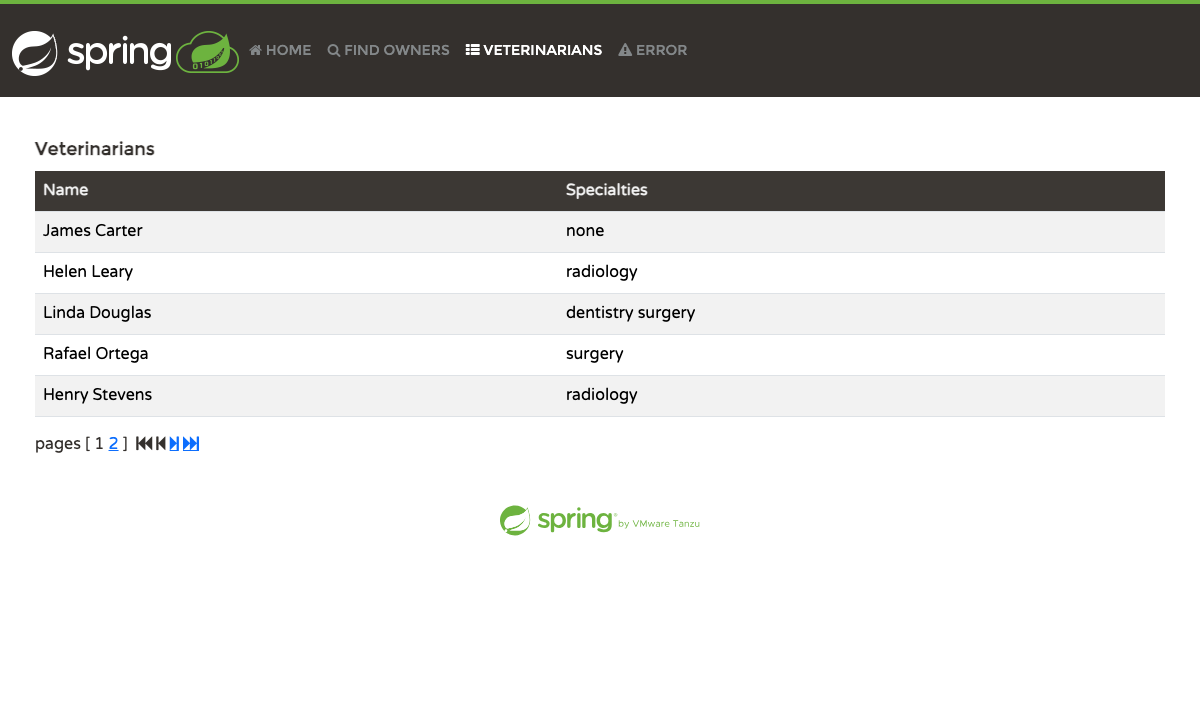
\includegraphics[width=0.58\linewidth]{assets/vets.png}
\caption{Veterinarians page served from the \code{vets} and \code{specialties} tables.}
\end{figure}

\chapter{CI/CD Pipeline}
The repository's own GitHub Actions workflow (\code{.github/workflows/maven-build.yml}) runs on
every push and pull request to \code{main}: it checks out the code, sets up JDK 17 with Maven
caching, and runs \code{./mvnw -B verify}. An equivalent Azure Pipelines definition for the
course (written for this report, \emph{not executed on Azure DevOps}) is below. Its stages are checkout and JDK setup, \code{verify} (compile, run all tests, package), and publishing test results so a failing test blocks the merge:

\begin{lstlisting}[language=bash]
trigger: [ main ]
pool: { vmImage: ubuntu-latest }
steps:
  - task: JavaToolInstaller@0
    inputs: { versionSpec: '17', jdkArchitectureOption: x64, jdkSourceOption: PreInstalled }
  - script: ./mvnw -B verify
    displayName: Build and test
  - task: PublishTestResults@2
    inputs: { testResultsFormat: JUnit, testResultsFiles: '**/surefire-reports/TEST-*.xml' }
\end{lstlisting}


\chapter{Conclusion}
Spring PetClinic shows how a small codebase can still apply the full construction toolkit:
clear layering, a compact domain model, SOLID-aligned class design, a test suite that maps to the
user stories (85 tests, all passing locally, including six added for the new pet-age feature) and a CI workflow that rebuilds and re-tests every
change. The report documents these from the actual source; the Azure Boards, Repos and
Pipelines screens were not captured because those services were not used for this submission.

\end{document}
